\documentclass{article}
\usepackage{tikz, comment}
\usepackage{pifont}
\usepackage{fontspec, pgfplots}
\usetikzlibrary{arrows, decorations.markings, decorations.pathreplacing}
\begin{comment}
:Title: Not defined yet
:Tags: absolute value rules;properties of equality, equation rules;set;equivalence properties of equality;trichotomy
:Prob: 0.6654;0.6065;0.5874;0.5808;0.57
:Author: Prof.Hu Ji-shan, HKUST
:Slug: No name yet

Description Here.........
\end{comment}
\begin{document}\centering 

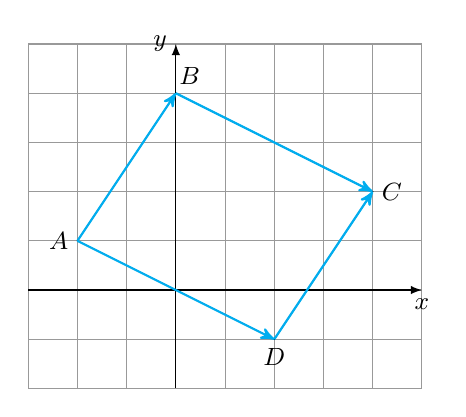
\begin{tikzpicture}[>=latex,xscale=.5*1.25, yscale=.5*1.25][font=\sf\small] 

\draw[xstep=1cm,ystep=1cm,color=gray!80] (-3, -2) grid (5, 5);

\draw[->] (-3, 0) -- (5, 0)node[below] {$x$} ;
\draw[->] (0, -2) -- (0, 5)node[left] {$y$} ;

\draw (-2, 1)node[left]{$A$} -- (0, 4)node[above, xshift = 5]{$B$} -- (4, 2)node[right]{$C$} -- (2, -1)node[below]{$D$} -- cycle;

\draw[cyan, thick, ->, >=stealth'] (-2, 1) -- (0, 4);
\draw[cyan, thick, ->, >=stealth'] (-2, 1) -- (2, -1);

\draw[cyan, thick, ->, >=stealth'] (0, 4) -- (4, 2);
\draw[cyan, thick, ->, >=stealth'] (2, -1) -- (4, 2);

\end{tikzpicture}
\end{document}